% Options for packages loaded elsewhere
\PassOptionsToPackage{unicode}{hyperref}
\PassOptionsToPackage{hyphens}{url}
\documentclass[
]{article}
\usepackage{xcolor}
\usepackage[margin=1in]{geometry}
\usepackage{amsmath,amssymb}
\setcounter{secnumdepth}{5}
\usepackage{iftex}
\ifPDFTeX
  \usepackage[T1]{fontenc}
  \usepackage[utf8]{inputenc}
  \usepackage{textcomp} % provide euro and other symbols
\else % if luatex or xetex
  \usepackage{unicode-math} % this also loads fontspec
  \defaultfontfeatures{Scale=MatchLowercase}
  \defaultfontfeatures[\rmfamily]{Ligatures=TeX,Scale=1}
\fi
\usepackage{lmodern}
\ifPDFTeX\else
  % xetex/luatex font selection
\fi
% Use upquote if available, for straight quotes in verbatim environments
\IfFileExists{upquote.sty}{\usepackage{upquote}}{}
\IfFileExists{microtype.sty}{% use microtype if available
  \usepackage[]{microtype}
  \UseMicrotypeSet[protrusion]{basicmath} % disable protrusion for tt fonts
}{}
\makeatletter
\@ifundefined{KOMAClassName}{% if non-KOMA class
  \IfFileExists{parskip.sty}{%
    \usepackage{parskip}
  }{% else
    \setlength{\parindent}{0pt}
    \setlength{\parskip}{6pt plus 2pt minus 1pt}}
}{% if KOMA class
  \KOMAoptions{parskip=half}}
\makeatother
\usepackage{color}
\usepackage{fancyvrb}
\newcommand{\VerbBar}{|}
\newcommand{\VERB}{\Verb[commandchars=\\\{\}]}
\DefineVerbatimEnvironment{Highlighting}{Verbatim}{commandchars=\\\{\}}
% Add ',fontsize=\small' for more characters per line
\usepackage{framed}
\definecolor{shadecolor}{RGB}{248,248,248}
\newenvironment{Shaded}{\begin{snugshade}}{\end{snugshade}}
\newcommand{\AlertTok}[1]{\textcolor[rgb]{0.94,0.16,0.16}{#1}}
\newcommand{\AnnotationTok}[1]{\textcolor[rgb]{0.56,0.35,0.01}{\textbf{\textit{#1}}}}
\newcommand{\AttributeTok}[1]{\textcolor[rgb]{0.13,0.29,0.53}{#1}}
\newcommand{\BaseNTok}[1]{\textcolor[rgb]{0.00,0.00,0.81}{#1}}
\newcommand{\BuiltInTok}[1]{#1}
\newcommand{\CharTok}[1]{\textcolor[rgb]{0.31,0.60,0.02}{#1}}
\newcommand{\CommentTok}[1]{\textcolor[rgb]{0.56,0.35,0.01}{\textit{#1}}}
\newcommand{\CommentVarTok}[1]{\textcolor[rgb]{0.56,0.35,0.01}{\textbf{\textit{#1}}}}
\newcommand{\ConstantTok}[1]{\textcolor[rgb]{0.56,0.35,0.01}{#1}}
\newcommand{\ControlFlowTok}[1]{\textcolor[rgb]{0.13,0.29,0.53}{\textbf{#1}}}
\newcommand{\DataTypeTok}[1]{\textcolor[rgb]{0.13,0.29,0.53}{#1}}
\newcommand{\DecValTok}[1]{\textcolor[rgb]{0.00,0.00,0.81}{#1}}
\newcommand{\DocumentationTok}[1]{\textcolor[rgb]{0.56,0.35,0.01}{\textbf{\textit{#1}}}}
\newcommand{\ErrorTok}[1]{\textcolor[rgb]{0.64,0.00,0.00}{\textbf{#1}}}
\newcommand{\ExtensionTok}[1]{#1}
\newcommand{\FloatTok}[1]{\textcolor[rgb]{0.00,0.00,0.81}{#1}}
\newcommand{\FunctionTok}[1]{\textcolor[rgb]{0.13,0.29,0.53}{\textbf{#1}}}
\newcommand{\ImportTok}[1]{#1}
\newcommand{\InformationTok}[1]{\textcolor[rgb]{0.56,0.35,0.01}{\textbf{\textit{#1}}}}
\newcommand{\KeywordTok}[1]{\textcolor[rgb]{0.13,0.29,0.53}{\textbf{#1}}}
\newcommand{\NormalTok}[1]{#1}
\newcommand{\OperatorTok}[1]{\textcolor[rgb]{0.81,0.36,0.00}{\textbf{#1}}}
\newcommand{\OtherTok}[1]{\textcolor[rgb]{0.56,0.35,0.01}{#1}}
\newcommand{\PreprocessorTok}[1]{\textcolor[rgb]{0.56,0.35,0.01}{\textit{#1}}}
\newcommand{\RegionMarkerTok}[1]{#1}
\newcommand{\SpecialCharTok}[1]{\textcolor[rgb]{0.81,0.36,0.00}{\textbf{#1}}}
\newcommand{\SpecialStringTok}[1]{\textcolor[rgb]{0.31,0.60,0.02}{#1}}
\newcommand{\StringTok}[1]{\textcolor[rgb]{0.31,0.60,0.02}{#1}}
\newcommand{\VariableTok}[1]{\textcolor[rgb]{0.00,0.00,0.00}{#1}}
\newcommand{\VerbatimStringTok}[1]{\textcolor[rgb]{0.31,0.60,0.02}{#1}}
\newcommand{\WarningTok}[1]{\textcolor[rgb]{0.56,0.35,0.01}{\textbf{\textit{#1}}}}
\usepackage{longtable,booktabs,array}
\usepackage{calc} % for calculating minipage widths
% Correct order of tables after \paragraph or \subparagraph
\usepackage{etoolbox}
\makeatletter
\patchcmd\longtable{\par}{\if@noskipsec\mbox{}\fi\par}{}{}
\makeatother
% Allow footnotes in longtable head/foot
\IfFileExists{footnotehyper.sty}{\usepackage{footnotehyper}}{\usepackage{footnote}}
\makesavenoteenv{longtable}
\usepackage{graphicx}
\makeatletter
\newsavebox\pandoc@box
\newcommand*\pandocbounded[1]{% scales image to fit in text height/width
  \sbox\pandoc@box{#1}%
  \Gscale@div\@tempa{\textheight}{\dimexpr\ht\pandoc@box+\dp\pandoc@box\relax}%
  \Gscale@div\@tempb{\linewidth}{\wd\pandoc@box}%
  \ifdim\@tempb\p@<\@tempa\p@\let\@tempa\@tempb\fi% select the smaller of both
  \ifdim\@tempa\p@<\p@\scalebox{\@tempa}{\usebox\pandoc@box}%
  \else\usebox{\pandoc@box}%
  \fi%
}
% Set default figure placement to htbp
\def\fps@figure{htbp}
\makeatother
\setlength{\emergencystretch}{3em} % prevent overfull lines
\providecommand{\tightlist}{%
  \setlength{\itemsep}{0pt}\setlength{\parskip}{0pt}}
\usepackage{booktabs}
\usepackage{float}
\usepackage{amsmath}
\floatplacement{figure}{H}
\usepackage{booktabs}
\usepackage{longtable}
\usepackage{array}
\usepackage{multirow}
\usepackage{wrapfig}
\usepackage{float}
\usepackage{colortbl}
\usepackage{pdflscape}
\usepackage{tabu}
\usepackage{threeparttable}
\usepackage{threeparttablex}
\usepackage[normalem]{ulem}
\usepackage{makecell}
\usepackage{xcolor}
\usepackage{bookmark}
\IfFileExists{xurl.sty}{\usepackage{xurl}}{} % add URL line breaks if available
\urlstyle{same}
\hypersetup{
  pdftitle={Project 2: Modelling daily cycling demand in Edinburgh},
  pdfauthor={Group members: Alice Miller, Saba Sitter, Jake Saunders},
  hidelinks,
  pdfcreator={LaTeX via pandoc}}

\title{Project 2: Modelling daily cycling demand in Edinburgh}
\author{Group members: Alice Miller, Saba Sitter, Jake Saunders}
\date{Word count: {[}XXX words{]}}

\begin{document}
\maketitle

\section{Introduction}\label{introduction}

The ``cycle daily'' dataset consists of approximately 2,180 daily
observations ranging from 2020 to 2025, sourced from Edinburgh's network
of automatic cycling counters, along with local weather and temporal
data. This data comes from sensors at specific locations across the
city, so it's possible not every cyclist is accounted for. Similarly,
some cyclists may pass through multiple sensors in a day and be observed
more than once. However, they are a good indicator of how cycling demand
varies across different days and weather patterns. Edinburgh relies
heavily on public transport for its residents and tourists to navigate
the city. For future funding allocation and planning, it is important to
know how many cyclists are on the road in order to evaluate whether the
infrastructure (cycle lanes, crossings etc) and investment in schemes
(eg rentable Voi bikes) need to adapt to meet demand. The modelling goal
is to develop a sequence of increasingly complex linear regression
models to isolate how temporal and weather variables, such as the day of
the week and the temperature, influence cycling demand. Ultimately, the
goal is to extrapolate cycling demand so that Edinburgh City Council and
Transport Scotland can optimise infrastructure investment over the next
decade to align with their active travel priorities.

\section{Exploratory data analysis}\label{exploratory-data-analysis}

To begin investigating the impact of weather on the number of daily
cyclists, we begun with some exploratory data analysis. This involved
converting month to an ordered factor, redefining the day of week
predictor with explicit levels. Additionally, we created a new variable
`trend' which symbolises the number of days since the first observation
(01/01/2020), along wtih binary indicators `is\_covid' and `is\_holiday'
which represent the UK Covid lockdown (23/03/2020 - 31/03/2021) and the
yearly festive period (24th - 31st December) respectively.

We initially found the summary statistics for the number of daily
cyclists and the weather data.

\begin{longtable}[]{@{}lrrrr@{}}
\caption{Summary Statistics for count, temp mean, temp min, temp
max}\tabularnewline
\toprule\noalign{}
Variable & Mean & SD & Min & Max \\
\midrule\noalign{}
\endfirsthead
\toprule\noalign{}
Variable & Mean & SD & Min & Max \\
\midrule\noalign{}
\endhead
\bottomrule\noalign{}
\endlastfoot
count & 10815.47 & 4728.88 & 1264.00 & 43864.00 \\
temp\_mean & 9.69 & 4.79 & -8.08 & 22.96 \\
temp\_min & 5.92 & 4.98 & -14.00 & 18.00 \\
temp\_max & 13.15 & 5.31 & -3.00 & 31.00 \\
\end{longtable}

We can see that the number of daily cyclists varies from \(1,264\) to
\(43,864\), a variation of \(\approx 3370 \%\). Intuitively, one would
think that a warmer average weather would lead to more cyclists.

We then plotted a time series of the daily cyclist count over the period
of observations.

\begin{figure}
\centering
\pandocbounded{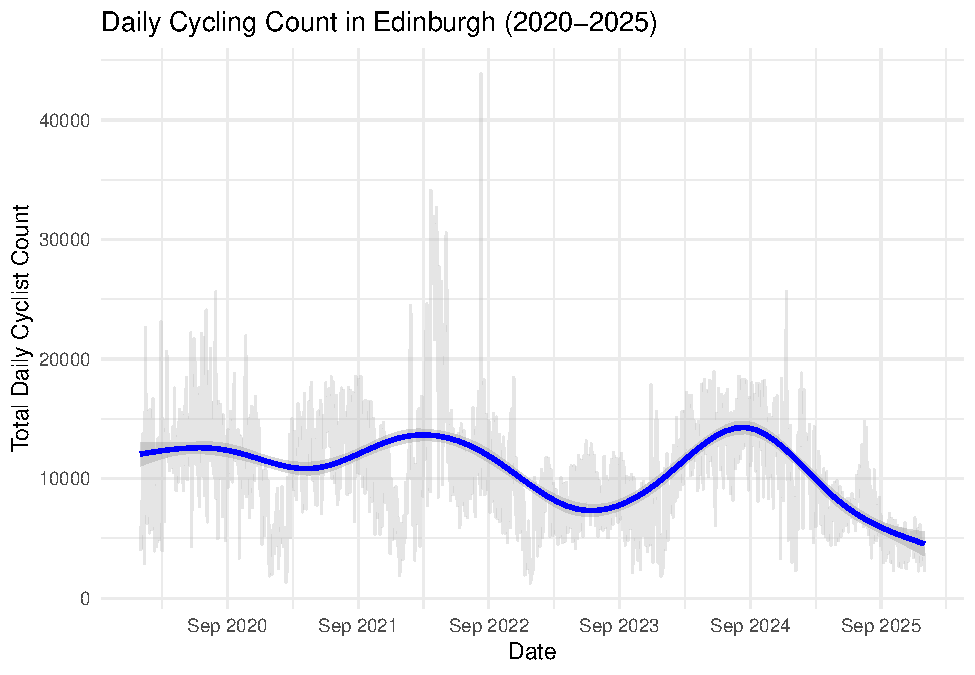
\includegraphics[keepaspectratio]{Report_project02_files/figure-latex/time series-1.pdf}}
\caption{Time series of daily cyclist counts 2020-2025}
\end{figure}

We can see from Figure X that there are yearly fluctuations, with peaks
and troughs occurring seasonally. Overall, the cyclist count seems to be
decreasing over time. There is a visible peak on and surrounding the
10th of August 2022, which we investigated. We found that there was a
London-Edinburgh-London bicycle event taking place over this period with
over 2000 riders\(^{1}\). Supposing each cyclist passed through multiple
sensors over the course of the days, this likely explains the inflated
numbers.

We then created boxplots of the daily cyclist count by month and by the
day of week to observe whether they had any significant impact on the
number of daily cyclists.

\begin{figure}
\centering
\pandocbounded{
\includegraphics[keepaspectratio]{Report_project02_files/figure-latex/Boxplots of cyclist count by month and day of week-1.pdf}}
\caption{Boxplots of cyclist count by month and day of week}
\end{figure}

We can see from Figure 2 that the colder months (October - February)
have slightly lower cyclist counts, with the other months remaining
relatively constant. There are a lot of outliers, especially in Spring.
Observations with unusually high cyclist counts could be attributed to
special events such as races, bank holidays, and exceptionally sunny
days. Outside of winter, the month doesn't appear to have a tremendous
impact on the median daily cyclist count.

The second boxplot indicates that there tends to be less cyclists on
Mondays and Sundays, with the other days appearing relatively constant.

We then plotted the daily cyclist count against the mean temperature,
with red and blue lines indicating regression and quadratic relationship
respectively.

\begin{figure}
\centering
\pandocbounded{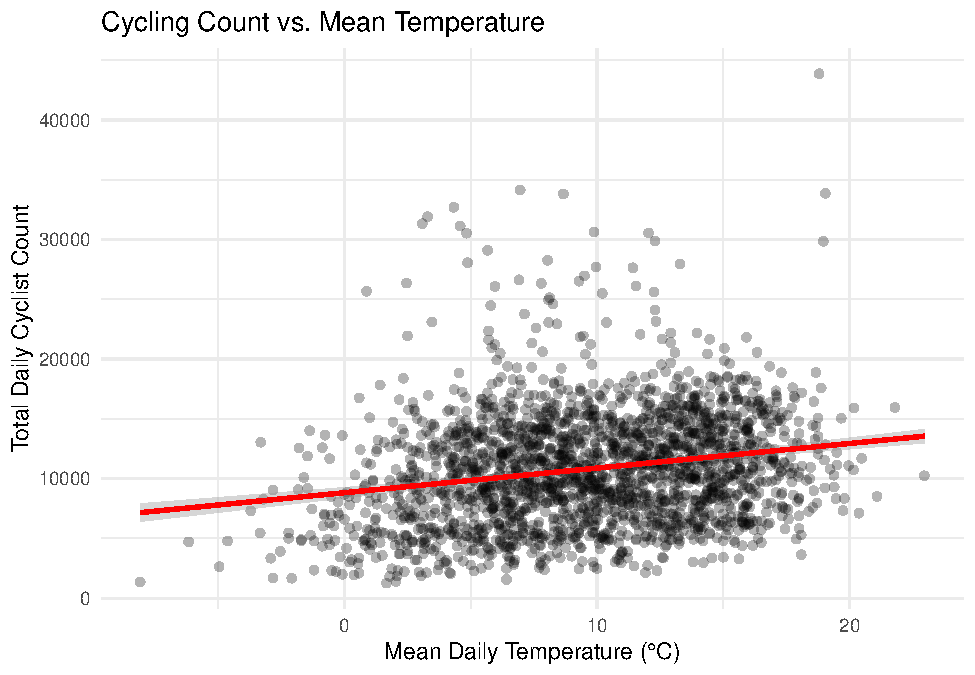
\includegraphics[keepaspectratio]{Report_project02_files/figure-latex/scatter plot of count vs temp_mean-1.pdf}}
\caption{Daily cyclist count vs mean temperature}
\end{figure}

There is a visible positive correlation between temperature mean and
daily cyclist count, which was to be expected. There are less
observations for the days with the lowest and highest mean temperatures,
so there is not a clear trend that we can see for those days. There is a
large variation in cyclist counts for days with the same temperature, so
it is not feasible to predict counts based off of mean temperature
alone.

We noticed dips in cyclist numbers between Christmas Eve and New Years
Eve, presumably due to less commuters on the road. We created the
following graph to illustrate this over the course of the 5 years.

\begin{figure}
\centering
\pandocbounded{
\includegraphics[keepaspectratio]{Report_project02_files/figure-latex/plot showing december-1.pdf}}
\caption{Daily cyclist count vs mean temperature}
\end{figure}

Clearly, there is a substantial decrease in cyclist numbers between the
specified days. This led us to add whether a day falls between the 24th
and 31st of December in our final model as `is\_holiday'.

We also created a chart that demonstrates the effect of whether a day is
lockdown on daily cyclist counts.

\section{Baseline model}\label{baseline-model}

We fit an initial model, M0, that uses the mean temperature, along with
the month and whether it is a weekend in order to predict the daily
cyclist count.

The equation for M0 is:

\#\[\text{count}_i = \beta_0 + \beta_1 \text{temp_mean}_i + \beta_2 \text{weekend}_i + \beta_3 \text{month}_i + \epsilon_i\]
\#\[\epsilon_i \sim N(0, \sigma^2)\]

The following table shows the summary statistics for M0:

\begin{longtable}[]{@{}
  >{\raggedright\arraybackslash}p{(\linewidth - 8\tabcolsep) * \real{0.2817}}
  >{\raggedleft\arraybackslash}p{(\linewidth - 8\tabcolsep) * \real{0.1549}}
  >{\raggedleft\arraybackslash}p{(\linewidth - 8\tabcolsep) * \real{0.1549}}
  >{\raggedleft\arraybackslash}p{(\linewidth - 8\tabcolsep) * \real{0.1408}}
  >{\raggedleft\arraybackslash}p{(\linewidth - 8\tabcolsep) * \real{0.2676}}@{}}
\caption{Summary of M0}\tabularnewline
\toprule\noalign{}
\begin{minipage}[b]{\linewidth}\raggedright
\end{minipage} & \begin{minipage}[b]{\linewidth}\raggedleft
Estimate
\end{minipage} & \begin{minipage}[b]{\linewidth}\raggedleft
Std. Error
\end{minipage} & \begin{minipage}[b]{\linewidth}\raggedleft
t value
\end{minipage} & \begin{minipage}[b]{\linewidth}\raggedleft
Pr(\textgreater\textbar t\textbar)
\end{minipage} \\
\midrule\noalign{}
\endfirsthead
\toprule\noalign{}
\begin{minipage}[b]{\linewidth}\raggedright
\end{minipage} & \begin{minipage}[b]{\linewidth}\raggedleft
Estimate
\end{minipage} & \begin{minipage}[b]{\linewidth}\raggedleft
Std. Error
\end{minipage} & \begin{minipage}[b]{\linewidth}\raggedleft
t value
\end{minipage} & \begin{minipage}[b]{\linewidth}\raggedleft
Pr(\textgreater\textbar t\textbar)
\end{minipage} \\
\midrule\noalign{}
\endhead
\bottomrule\noalign{}
\endlastfoot
(Intercept) & 10385.8188 & 267.01547 & 38.895944 & 0 \\
temp\_mean & 247.1791 & 20.76877 & 11.901478 & 0 \\
as.numeric(weekend) & -1246.8883 & 214.17220 & -5.821896 & 0 \\
as.numeric(month) & -247.1840 & 28.80970 & -8.579887 & 0 \\
\end{longtable}

For every 1 degree increase in the mean daily temperature, the model
predicts an increase of 247 cyclists per day, and predicts a 1247
decrease in cyclist count on weekends compared to weekdays. Since M0
uses month as a numeric predictor, it ignores the fact that cyclist
counts generally increase in summer and fall in winter. Currently, the
model suggests that there is a decrease of 247 cyclists for each month
passing.

We then assessed the diagnostic plots for M0.

\pandocbounded{\includegraphics[keepaspectratio]{Report_project02_files/figure-latex/r vs f and qq plots m0-1.pdf}}
\pandocbounded{\includegraphics[keepaspectratio]{Report_project02_files/figure-latex/r vs f and qq plots m0-2.pdf}}
The Normal

Model 0 (m0) shows a mean variance of 0, independent of the fitted
values. The residuals show a non-linear pattern, with an arguable `n'
shape above the mean line, indicating there is an underlying non-linear
structure yet to be included in our model.

The QQ plot demonstrates right skewing and heavy tail in the positive
quantiles - thus the normality assumption for linear regression is
violated. This indicates the model is particularly bad at predicting
high count observations.

\section{Model M1}\label{model-m1}

We created a further model, M1, which adds in the trend variable as a
predictor to capture the drift in cycling levels over 2020-2025. We
switched month and day of week to factor variables, so each level gets
its own intercept.

Our proposed equation for M1 is:
\[\text{count}_i = \beta_0 + \beta_1 \text{temp_mean}_i + \beta_2 \text{trend}_i + \beta_k \text{month}_i + \beta_j \text{dow}_i +  \epsilon_i\]
\[\epsilon_i \sim N(0, \sigma^2), k \in \{1,...,12 \}, j \in \{1,...,7 \} \]

Rational for investigating m1 over m0: m1 has the granularity for the
effect of different weekdays rather than mere weekend or non weekend
effects. Changing `month' to a factor variable allows for building a
seasonal profile rather than assuming the month index (1-12) is linear
with the count.

We omit the weekend term and numerical version of month to avoid
collinearity with their `factor' versions and because the covariate dow
is collinear with weekend.

\pandocbounded{\includegraphics[keepaspectratio]{Report_project02_files/figure-latex/side by side comparison of M0 and M1-1.pdf}}

Observe in the bottom left: the mean residual line follows a sigmoid
shape, suggesting the linear assumption is still violated for model 1.
On a positive note, the `n' pattern is less pronounced for model 1. The
bottom right Q-Q plot looks slightly more aligned to the normal line at
the lower tail (compared to M0), which suggests the prediction for low
count days is better.

\subsection{Model M2: Nonlinear
temperature}\label{model-m2-nonlinear-temperature}

Observe from the temperature vs count scatter plot, there is some non
linear relationship as we can see some curvature (blue line). Hence, if
we add the quadratic `mean temperature' term to model m1, the underlying
structure maybe better covered by the model:

\pandocbounded{\includegraphics[keepaspectratio]{Report_project02_files/figure-latex/thing-1.pdf}}
M2 shows a general allignment with linear modelling assumptions - no big
violations. Observe that both models look almost identical from the
diagnostic plots, which indicates further comparison may be undertaken
using the scores.

\subsection{Model M3: {[}your extension
title{]}}\label{model-m3-your-extension-title}

\begin{longtable}[]{@{}
  >{\raggedright\arraybackslash}p{(\linewidth - 0\tabcolsep) * \real{0.0833}}@{}}
\toprule\noalign{}
\endhead
\bottomrule\noalign{}
\endlastfoot
IDEATION: If your primary goal is to fix the plots you just showed
me: \\
Choose the Log-transform to fix the Q-Q plot (the outliers). \\
Choose the Interaction or Temperature Range to fix the Residuals vs
Fitted (the ``wiggle''). \\
\end{longtable}

\section{Evaluation}\label{evaluation}

\subsection{Statistical Performance}\label{statistical-performance}

Table of the Leave-one-year-out CV scores.

\begin{longtable}[]{@{}lrrrr@{}}
\caption{Table of the Leave-one-year-out CV scores}\tabularnewline
\toprule\noalign{}
Model & RMSE & MAE & DS & IS \\
\midrule\noalign{}
\endfirsthead
\toprule\noalign{}
Model & RMSE & MAE & DS & IS \\
\midrule\noalign{}
\endhead
\bottomrule\noalign{}
\endlastfoot
m0 & 4740.88 & 3805.56 & 18.05 & 25630.46 \\
m1 & 4587.61 & 3650.23 & 18.07 & 25277.87 \\
m2 & 4587.61 & 3650.23 & 18.07 & 25277.87 \\
m3 & 4847.43 & 3917.76 & 19.06 & 34538.19 \\
\end{longtable}

Table of the RMSE and DS by month

\begin{longtable}[]{@{}lrr@{}}
\caption{Table of the RMSE and DS by months}\tabularnewline
\toprule\noalign{}
Month & RMSE & DS \\
\midrule\noalign{}
\endfirsthead
\toprule\noalign{}
Month & RMSE & DS \\
\midrule\noalign{}
\endhead
\bottomrule\noalign{}
\endlastfoot
Jan & 4141.9 & 18.25 \\
Feb & 3518.0 & 17.53 \\
Mar & 5126.4 & 18.10 \\
Apr & 5437.0 & 18.43 \\
May & 4372.4 & 17.79 \\
Jun & 3162.2 & 17.32 \\
Jul & 3118.6 & 17.19 \\
Aug & 4408.1 & 17.71 \\
Sep & 3182.2 & 17.31 \\
Oct & 3357.9 & 17.47 \\
Nov & 3512.2 & 17.59 \\
Dec & 3574.1 & 18.64 \\
\end{longtable}

\subsection{Practical Performance}\label{practical-performance}

\subsubsection{5.1 Temperature effects and
nonlinearlity}\label{temperature-effects-and-nonlinearlity}

The table shows the different score values for model 2, but using 3
different temperature variables:temp mean, temp min and temp max.

\begin{longtable}[]{@{}lrrrr@{}}
\caption{Model M2 fitted with daily temp mean, temp min, temp
max.}\tabularnewline
\toprule\noalign{}
Model & RMSE & MAE & DS & IS \\
\midrule\noalign{}
\endfirsthead
\toprule\noalign{}
Model & RMSE & MAE & DS & IS \\
\midrule\noalign{}
\endhead
\bottomrule\noalign{}
\endlastfoot
Temp Mean & 5459.30 & 4202.82 & 18.46 & 31740.12 \\
Temp Min & 5475.41 & 4216.60 & 18.48 & 31929.26 \\
Temp Max & 5453.76 & 4202.23 & 18.46 & 31560.07 \\
\end{longtable}

The model with temp max in the nonlinear term has the best predictive
performance because it has the lowest value for each score.

At \(5 ^\circ\) c,a \(1 ^\circ\) c increase is associated with
approximately 108 additional cyclists.

At \(15 ^\circ\) c,a \(1 ^\circ\) c increase is associated with
approximately 166 additional cyclists.

We can see the effects a \(1 ^\circ\) increase has in Spring and winter
specifically.

On a Spring day at \(5 ^\circ\) c,a \(1 ^\circ\) c increase is
associated with approximately 343 additional cyclists.

On a Spring day at \(15 ^\circ\) c,a \(1 ^\circ\) c increase is
associated with approximately 424 additional cyclists.

On a Winters day at \(5 ^\circ\) c,a \(1 ^\circ\) c increase is
associated with approximately 56 additional cyclists.

On a Winters day at \(15 ^\circ\) c,a \(1 ^\circ\) c increase is
associated with approximately 137 additional cyclists.

As we can see, there is huge variablity between seasons. For transport
planning this implies that looking at the range of temperatures for the
day is more importantas it will have a bigger effect.

\section{Discussion and limitations}\label{discussion-and-limitations}

\section{Appendix - References}\label{appendix---references}

\(^{1}\)
\url{https://mccyclingdiary.blogspot.com/2022/08/london-edinburg-london-lel-2022-edition.html}

\section{Appendix - Code}\label{appendix---code}

All analysis code is in \texttt{code.R} and is reproduced below.

\begin{Shaded}
\begin{Highlighting}[]
\CommentTok{\# ============================================================}
\CommentTok{\# Project 2: Modelling daily cycling demand in Edinburgh}
\CommentTok{\# Authors: Alice Miller, Saba Sitter, Jake Saunders}
\CommentTok{\# ============================================================}

\CommentTok{\#}
\CommentTok{\# Place the code needed in the Report\_project02.Rmd, including documentation.}
\CommentTok{\#}
\CommentTok{\# 0. Packages}
\FunctionTok{library}\NormalTok{(ggplot2); }\FunctionTok{library}\NormalTok{(dplyr); }\FunctionTok{library}\NormalTok{(tidyr)}
\FunctionTok{library}\NormalTok{(lubridate); }\FunctionTok{library}\NormalTok{(knitr); }\FunctionTok{library}\NormalTok{(kableExtra)}
\FunctionTok{library}\NormalTok{(patchwork); }\FunctionTok{library}\NormalTok{(broom); }\FunctionTok{library}\NormalTok{(gridExtra)}

\CommentTok{\# 1. Load data}
\FunctionTok{load}\NormalTok{(}\StringTok{\textquotesingle{}cycle\_daily\_df.Rdata\textquotesingle{}}\NormalTok{)}

\CommentTok{\# 2.1 Data Wrangling }
\NormalTok{cycle\_daily\_df }\OtherTok{\textless{}{-}}\NormalTok{ cycle\_daily\_df }\SpecialCharTok{\%\textgreater{}\%}
  \FunctionTok{mutate}\NormalTok{(}
    
    \CommentTok{\#Season indicator}
    \AttributeTok{m\_num =} \FunctionTok{month}\NormalTok{(date),}
    \AttributeTok{is\_spring =} \FunctionTok{ifelse}\NormalTok{(m\_num }\SpecialCharTok{\%in\%} \DecValTok{3}\SpecialCharTok{:}\DecValTok{5}\NormalTok{, }\DecValTok{1}\NormalTok{, }\DecValTok{0}\NormalTok{),}
    \AttributeTok{is\_summer =} \FunctionTok{ifelse}\NormalTok{(m\_num }\SpecialCharTok{\%in\%} \DecValTok{6}\SpecialCharTok{:}\DecValTok{8}\NormalTok{, }\DecValTok{1}\NormalTok{, }\DecValTok{0}\NormalTok{),}
    \AttributeTok{is\_autumn =} \FunctionTok{ifelse}\NormalTok{(m\_num }\SpecialCharTok{\%in\%} \DecValTok{9}\SpecialCharTok{:}\DecValTok{11}\NormalTok{, }\DecValTok{1}\NormalTok{, }\DecValTok{0}\NormalTok{),}
    \AttributeTok{is\_winter =} \FunctionTok{ifelse}\NormalTok{(m\_num }\SpecialCharTok{\%in\%} \FunctionTok{c}\NormalTok{(}\DecValTok{12}\NormalTok{, }\DecValTok{1}\NormalTok{, }\DecValTok{2}\NormalTok{), }\DecValTok{1}\NormalTok{, }\DecValTok{0}\NormalTok{),}
    
    \CommentTok{\# Task 2: dow with explicit levels }
    \AttributeTok{dow =} \FunctionTok{factor}\NormalTok{(dow,}
                 \AttributeTok{levels =} \FunctionTok{c}\NormalTok{(}\StringTok{"Mon"}\NormalTok{, }\StringTok{"Tue"}\NormalTok{, }\StringTok{"Wed"}\NormalTok{, }\StringTok{"Thu"}\NormalTok{, }\StringTok{"Fri"}\NormalTok{, }\StringTok{"Sat"}\NormalTok{, }\StringTok{"Sun"}\NormalTok{), }
                 \AttributeTok{ordered =} \ConstantTok{TRUE}\NormalTok{),}
    
    \CommentTok{\# Task 3: trend as integer days since 2020{-}01{-}01}
    \AttributeTok{trend =} \FunctionTok{as.numeric}\NormalTok{(date }\SpecialCharTok{{-}}\NormalTok{ date[}\DecValTok{1}\NormalTok{], }\AttributeTok{units =} \StringTok{"days"}\NormalTok{),}
    
    \CommentTok{\#Covid indicator}
    \AttributeTok{is\_covid =} \FunctionTok{ifelse}\NormalTok{(date }\SpecialCharTok{\textgreater{}=} \StringTok{"2020{-}03{-}23"} \SpecialCharTok{\&}\NormalTok{ date }\SpecialCharTok{\textless{}=} \StringTok{"2021{-}03{-}31"}\NormalTok{,}\DecValTok{1}\NormalTok{,}\DecValTok{0}\NormalTok{),}
    
    \CommentTok{\#festive period indicator}
    \AttributeTok{is\_holiday =} \FunctionTok{ifelse}\NormalTok{(m\_num }\SpecialCharTok{==} \DecValTok{12} \SpecialCharTok{\&} \FunctionTok{day}\NormalTok{(date) }\SpecialCharTok{\textgreater{}=}\DecValTok{24} \SpecialCharTok{\&} \FunctionTok{day}\NormalTok{(date)}\SpecialCharTok{\textless{}=}\DecValTok{31}\NormalTok{, }\DecValTok{1}\NormalTok{,}\DecValTok{0}\NormalTok{),}
    
    \CommentTok{\#Daily temp range}
    \AttributeTok{temp\_range =}\NormalTok{ temp\_max }\SpecialCharTok{{-}}\NormalTok{ temp\_min,}
    
    \CommentTok{\#cold indicator}
    \AttributeTok{is\_freezing =} \FunctionTok{ifelse}\NormalTok{(temp\_min }\SpecialCharTok{\textless{}=} \DecValTok{0}\NormalTok{, }\DecValTok{1}\NormalTok{, }\DecValTok{0}\NormalTok{))}\SpecialCharTok{\%\textgreater{}\%}
  
  \FunctionTok{mutate}\NormalTok{(}
    
    \CommentTok{\# Task 1: month as ordered factor for plots/inference}
    \AttributeTok{month =} \FunctionTok{factor}\NormalTok{(m\_num,}
                    \AttributeTok{levels =} \DecValTok{1}\SpecialCharTok{:}\DecValTok{12}\NormalTok{,    }
                    \AttributeTok{labels =}\NormalTok{ month.abb, }
                    \AttributeTok{ordered =} \ConstantTok{TRUE}\NormalTok{)}
    
\NormalTok{    )}

\CommentTok{\# 2.2 exploratory plots}

\CommentTok{\# Summary table for count, temp\_mean, temp\_min, temp\_max}
\NormalTok{summary\_stats }\OtherTok{\textless{}{-}}\NormalTok{ cycle\_daily\_df }\SpecialCharTok{\%\textgreater{}\%}
  \FunctionTok{summarise}\NormalTok{(}\FunctionTok{across}\NormalTok{(}\FunctionTok{c}\NormalTok{(count, temp\_mean, temp\_min, temp\_max), }
                   \FunctionTok{list}\NormalTok{(}\AttributeTok{Mean =} \SpecialCharTok{\textasciitilde{}}\FunctionTok{mean}\NormalTok{(.x), }
                        \AttributeTok{SD =} \SpecialCharTok{\textasciitilde{}}\FunctionTok{sd}\NormalTok{(.x), }
                        \AttributeTok{Min =} \SpecialCharTok{\textasciitilde{}}\FunctionTok{min}\NormalTok{(.x), }
                        \AttributeTok{Max =} \SpecialCharTok{\textasciitilde{}}\FunctionTok{max}\NormalTok{(.x)),}
                   \AttributeTok{.names =} \StringTok{"\{.col\}.\{.fn\}"}\NormalTok{)) }\SpecialCharTok{\%\textgreater{}\%} \CommentTok{\# use dots in variable names instead of underscore}
  \CommentTok{\# Reshape for a vertical table}
  \FunctionTok{pivot\_longer}\NormalTok{(}\FunctionTok{everything}\NormalTok{(), }
               \AttributeTok{names\_to =} \FunctionTok{c}\NormalTok{(}\StringTok{"Variable"}\NormalTok{, }\StringTok{"Statistic"}\NormalTok{), }
               \AttributeTok{names\_sep =} \StringTok{"}\SpecialCharTok{\textbackslash{}\textbackslash{}}\StringTok{."}\NormalTok{) }\SpecialCharTok{\%\textgreater{}\%} \CommentTok{\# Split at the dot instead of the underscore}
  \FunctionTok{pivot\_wider}\NormalTok{(}\AttributeTok{names\_from =}\NormalTok{ Statistic, }\AttributeTok{values\_from =}\NormalTok{ value)}


\CommentTok{\# Time series of daily counts 2020{-}2025 with a smoother}
\NormalTok{plot\_timeseries }\OtherTok{\textless{}{-}} \FunctionTok{ggplot}\NormalTok{(cycle\_daily\_df, }\FunctionTok{aes}\NormalTok{(}\AttributeTok{x =}\NormalTok{ date, }\AttributeTok{y =}\NormalTok{ count)) }\SpecialCharTok{+}
  \FunctionTok{geom\_line}\NormalTok{(}\AttributeTok{alpha =} \FloatTok{0.4}\NormalTok{, }\AttributeTok{color =} \StringTok{"gray"}\NormalTok{) }\SpecialCharTok{+} 
  \FunctionTok{geom\_smooth}\NormalTok{(}\AttributeTok{method =} \StringTok{"gam"}\NormalTok{, }\AttributeTok{color =} \StringTok{"blue"}\NormalTok{, }\AttributeTok{se =} \ConstantTok{TRUE}\NormalTok{) }\SpecialCharTok{+} \CommentTok{\# The smoother line}
  \FunctionTok{scale\_x\_date}\NormalTok{(}\AttributeTok{date\_breaks =} \StringTok{"12 months"}\NormalTok{, }\AttributeTok{date\_labels =} \StringTok{"\%b \%Y"}\NormalTok{) }\SpecialCharTok{+} 
  \FunctionTok{labs}\NormalTok{(}
    \AttributeTok{title =} \StringTok{"Daily Cycling Count in Edinburgh (2020{-}2025)"}\NormalTok{,}
    \AttributeTok{x =} \StringTok{"Date"}\NormalTok{,}
    \AttributeTok{y =} \StringTok{"Total Daily Cyclist Count"}
\NormalTok{  ) }\SpecialCharTok{+}
  \FunctionTok{theme\_minimal}\NormalTok{()}

\CommentTok{\# Boxplots of count by month and by day of week.}

\CommentTok{\# Boxplot by Month }
\NormalTok{plot\_month }\OtherTok{\textless{}{-}} \FunctionTok{ggplot}\NormalTok{(cycle\_daily\_df, }\FunctionTok{aes}\NormalTok{(}\AttributeTok{x =}\NormalTok{ month, }\AttributeTok{y =}\NormalTok{ count)) }\SpecialCharTok{+} \CommentTok{\# Use fill = month to add colour}
  \FunctionTok{geom\_boxplot}\NormalTok{(}\AttributeTok{show.legend =} \ConstantTok{FALSE}\NormalTok{) }\SpecialCharTok{+}
  \FunctionTok{labs}\NormalTok{(}\AttributeTok{title =} \StringTok{"Cycling Demand by Month"}\NormalTok{, }\AttributeTok{x =} \StringTok{"Month"}\NormalTok{, }\AttributeTok{y =} \StringTok{"Count"}\NormalTok{) }\SpecialCharTok{+}
  \FunctionTok{theme\_minimal}\NormalTok{()}

\CommentTok{\# Boxplot by Day of Week}
\NormalTok{plot\_dow }\OtherTok{\textless{}{-}} \FunctionTok{ggplot}\NormalTok{(cycle\_daily\_df, }\FunctionTok{aes}\NormalTok{(}\AttributeTok{x =}\NormalTok{ dow, }\AttributeTok{y =}\NormalTok{ count)) }\SpecialCharTok{+}
  \FunctionTok{geom\_boxplot}\NormalTok{(}\AttributeTok{show.legend =} \ConstantTok{FALSE}\NormalTok{) }\SpecialCharTok{+}
  \FunctionTok{labs}\NormalTok{(}\AttributeTok{title =} \StringTok{"Cycling Demand by Day of Week"}\NormalTok{, }\AttributeTok{x =} \StringTok{"Day"}\NormalTok{, }\AttributeTok{y =} \StringTok{"Count"}\NormalTok{) }\SpecialCharTok{+}
  \FunctionTok{theme\_minimal}\NormalTok{()}

\CommentTok{\# Scatter plot of count vs mean temperature}
\NormalTok{plot\_temp\_scatter }\OtherTok{\textless{}{-}} \FunctionTok{ggplot}\NormalTok{(cycle\_daily\_df, }\FunctionTok{aes}\NormalTok{(}\AttributeTok{x =}\NormalTok{ temp\_mean, }\AttributeTok{y =}\NormalTok{ count)) }\SpecialCharTok{+}
  \FunctionTok{geom\_point}\NormalTok{(}\AttributeTok{alpha =} \FloatTok{0.3}\NormalTok{) }\SpecialCharTok{+} \CommentTok{\# alpha changes the opaqueness of the points}
  \FunctionTok{geom\_smooth}\NormalTok{(}\AttributeTok{method =} \StringTok{"lm"}\NormalTok{, }\AttributeTok{color =} \StringTok{"red"}\NormalTok{, }\AttributeTok{se =} \ConstantTok{TRUE}\NormalTok{)}\SpecialCharTok{+}
  \FunctionTok{geom\_smooth}\NormalTok{(}\AttributeTok{method =} \StringTok{"lm"}\NormalTok{, }\AttributeTok{formula =}\NormalTok{ y }\SpecialCharTok{\textasciitilde{}}\NormalTok{ x }\SpecialCharTok{+} \FunctionTok{I}\NormalTok{(x}\SpecialCharTok{\^{}}\DecValTok{2}\NormalTok{), }\AttributeTok{color =} \StringTok{"blue"}\NormalTok{) }\SpecialCharTok{+}
  \FunctionTok{labs}\NormalTok{(}
    \AttributeTok{title =} \StringTok{"Cycling Count vs. Mean Temperature"}\NormalTok{,}
    \AttributeTok{x =} \StringTok{"Mean Daily Temperature (°C)"}\NormalTok{,}
    \AttributeTok{y =} \StringTok{"Total Daily Cyclist Count"}
\NormalTok{  ) }\SpecialCharTok{+}
  \FunctionTok{theme\_minimal}\NormalTok{()}

\CommentTok{\# non trivial plot {-} festive period}
\CommentTok{\# Filter for December and calculate the average count for each day across all years}
\NormalTok{december\_trends }\OtherTok{\textless{}{-}}\NormalTok{ cycle\_daily\_df }\SpecialCharTok{\%\textgreater{}\%}
  \FunctionTok{filter}\NormalTok{(}\FunctionTok{month}\NormalTok{(date) }\SpecialCharTok{==} \DecValTok{12}\NormalTok{) }\SpecialCharTok{\%\textgreater{}\%}
  \FunctionTok{mutate}\NormalTok{(}\AttributeTok{day =} \FunctionTok{day}\NormalTok{(date)) }\SpecialCharTok{\%\textgreater{}\%}
  \FunctionTok{group\_by}\NormalTok{(day) }\SpecialCharTok{\%\textgreater{}\%}
  \FunctionTok{summarise}\NormalTok{(}\AttributeTok{avg\_count =} \FunctionTok{mean}\NormalTok{(count, }\AttributeTok{na.rm =} \ConstantTok{TRUE}\NormalTok{),}
            \AttributeTok{sd\_count =} \FunctionTok{sd}\NormalTok{(count, }\AttributeTok{na.rm =} \ConstantTok{TRUE}\NormalTok{))}

\CommentTok{\# Create the plot}
\NormalTok{plot\_december }\OtherTok{\textless{}{-}}\FunctionTok{ggplot}\NormalTok{(december\_trends, }\FunctionTok{aes}\NormalTok{(}\AttributeTok{x =}\NormalTok{ day, }\AttributeTok{y =}\NormalTok{ avg\_count)) }\SpecialCharTok{+}
  \FunctionTok{geom\_line}\NormalTok{(}\AttributeTok{size =} \DecValTok{1}\NormalTok{) }\SpecialCharTok{+}
  \FunctionTok{labs}\NormalTok{(}\AttributeTok{title =} \StringTok{"Average Cycling Demand in December"}\NormalTok{,}
       \AttributeTok{subtitle =} \StringTok{"Average daily counts across 2020{-}2024"}\NormalTok{,}
       \AttributeTok{x =} \StringTok{"Day in December"}\NormalTok{,}
       \AttributeTok{y =} \StringTok{"Average Daily Cyclists"}\NormalTok{) }\SpecialCharTok{+}
  \FunctionTok{theme\_minimal}\NormalTok{()}

\CommentTok{\# 3. Model Fitting}
\CommentTok{\# Note: Use factor(month) in formulas for M1{-}M3}
\NormalTok{m0 }\OtherTok{\textless{}{-}} \FunctionTok{lm}\NormalTok{(count }\SpecialCharTok{\textasciitilde{}}\NormalTok{ temp\_mean }\SpecialCharTok{+} \FunctionTok{as.numeric}\NormalTok{(weekend) }\SpecialCharTok{+} \FunctionTok{as.numeric}\NormalTok{(month), }
         \AttributeTok{data =}\NormalTok{ cycle\_daily\_df)}

\DocumentationTok{\#\#m1\_literal has collinear terms so we define the factor versions of month and }
\CommentTok{\#dow and omit the weekend.}

\NormalTok{m1 }\OtherTok{\textless{}{-}} \FunctionTok{lm}\NormalTok{(count }\SpecialCharTok{\textasciitilde{}}\NormalTok{ temp\_mean }\SpecialCharTok{+}\NormalTok{ trend }\SpecialCharTok{+} \FunctionTok{factor}\NormalTok{(month) }\SpecialCharTok{+} \FunctionTok{factor}\NormalTok{(dow), }
         \AttributeTok{data =}\NormalTok{ cycle\_daily\_df)}

\NormalTok{m2 }\OtherTok{\textless{}{-}} \FunctionTok{lm}\NormalTok{(count }\SpecialCharTok{\textasciitilde{}}\NormalTok{ temp\_mean }\SpecialCharTok{+} \FunctionTok{I}\NormalTok{(temp\_mean}\SpecialCharTok{\^{}}\DecValTok{2}\NormalTok{)  }\SpecialCharTok{+}\NormalTok{ trend }\SpecialCharTok{+} 
           \FunctionTok{factor}\NormalTok{(month) }\SpecialCharTok{+} \FunctionTok{factor}\NormalTok{(dow), }\AttributeTok{data =}\NormalTok{ cycle\_daily\_df )}

\NormalTok{m3 }\OtherTok{\textless{}{-}} \FunctionTok{lm}\NormalTok{(}\FunctionTok{log}\NormalTok{(count}\SpecialCharTok{+}\DecValTok{1}\NormalTok{) }\SpecialCharTok{\textasciitilde{}}\NormalTok{ temp\_mean }\SpecialCharTok{+} \FunctionTok{I}\NormalTok{(temp\_mean}\SpecialCharTok{\^{}}\DecValTok{2}\NormalTok{) }\SpecialCharTok{+}\NormalTok{ trend }\SpecialCharTok{+} 
               \FunctionTok{factor}\NormalTok{(month) }\SpecialCharTok{+} \FunctionTok{factor}\NormalTok{(dow)  }\SpecialCharTok{+}\NormalTok{ is\_covid }\SpecialCharTok{+}\NormalTok{ is\_holiday, }\AttributeTok{data =}\NormalTok{ cycle\_daily\_df)}

\CommentTok{\#m0}
\CommentTok{\# Add residuals and fitted values to the dataframe.}
\NormalTok{m0\_diag }\OtherTok{\textless{}{-}} \FunctionTok{augment}\NormalTok{(m0)}

\CommentTok{\# Plot Residuals vs Fitted for m0}
\NormalTok{p1\_m0 }\OtherTok{\textless{}{-}} \FunctionTok{ggplot}\NormalTok{(m0\_diag, }\FunctionTok{aes}\NormalTok{(}\AttributeTok{x =}\NormalTok{ .fitted, }\AttributeTok{y =}\NormalTok{ .resid)) }\SpecialCharTok{+}
  \FunctionTok{geom\_point}\NormalTok{(}\AttributeTok{alpha =} \FloatTok{0.5}\NormalTok{) }\SpecialCharTok{+}
  \FunctionTok{geom\_hline}\NormalTok{(}\AttributeTok{yintercept =} \DecValTok{0}\NormalTok{, }\AttributeTok{linetype =} \StringTok{"dashed"}\NormalTok{, }\AttributeTok{color =} \StringTok{"red"}\NormalTok{) }\SpecialCharTok{+}
  \FunctionTok{geom\_smooth}\NormalTok{(}\AttributeTok{method =} \StringTok{"loess"}\NormalTok{, }\AttributeTok{se =} \ConstantTok{FALSE}\NormalTok{, }\AttributeTok{color =} \StringTok{"blue"}\NormalTok{) }\SpecialCharTok{+}
  \FunctionTok{labs}\NormalTok{(}\AttributeTok{title =} \StringTok{"Residuals vs Fitted"}\NormalTok{,}
       \AttributeTok{x =} \StringTok{"Fitted Values"}\NormalTok{,}
       \AttributeTok{y =} \StringTok{"Residuals"}\NormalTok{) }\SpecialCharTok{+}
  \FunctionTok{theme\_minimal}\NormalTok{()}

\CommentTok{\# Plot Normal Q{-}Q for m0}
\NormalTok{p2\_m0 }\OtherTok{\textless{}{-}} \FunctionTok{ggplot}\NormalTok{(m0\_diag, }\FunctionTok{aes}\NormalTok{(}\AttributeTok{sample =}\NormalTok{ .resid)) }\SpecialCharTok{+}
  \FunctionTok{stat\_qq}\NormalTok{(}\AttributeTok{alpha =} \FloatTok{0.5}\NormalTok{) }\SpecialCharTok{+}
  \FunctionTok{stat\_qq\_line}\NormalTok{(}\AttributeTok{color =} \StringTok{"red"}\NormalTok{) }\SpecialCharTok{+}
  \FunctionTok{labs}\NormalTok{(}\AttributeTok{title =} \StringTok{"Normal Q{-}Q Plot"}\NormalTok{,}
       \AttributeTok{x =} \StringTok{"Theoretical Quantiles"}\NormalTok{,}
       \AttributeTok{y =} \StringTok{"Sample Quantiles"}\NormalTok{) }\SpecialCharTok{+}
  \FunctionTok{theme\_minimal}\NormalTok{()}

\CommentTok{\# m1 }
\CommentTok{\# Add residuals and fitted values to the dataframe.}
\NormalTok{m1\_diag }\OtherTok{\textless{}{-}} \FunctionTok{augment}\NormalTok{(m1)}

\CommentTok{\# Residuals vs Fitted for M1}
\NormalTok{p1\_m1 }\OtherTok{\textless{}{-}} \FunctionTok{ggplot}\NormalTok{(m1\_diag, }\FunctionTok{aes}\NormalTok{(}\AttributeTok{x =}\NormalTok{ .fitted, }\AttributeTok{y =}\NormalTok{ .resid)) }\SpecialCharTok{+}
  \FunctionTok{geom\_point}\NormalTok{(}\AttributeTok{alpha =} \FloatTok{0.4}\NormalTok{) }\SpecialCharTok{+}
  \FunctionTok{geom\_hline}\NormalTok{(}\AttributeTok{yintercept =} \DecValTok{0}\NormalTok{, }\AttributeTok{linetype =} \StringTok{"dashed"}\NormalTok{, }\AttributeTok{color =} \StringTok{"red"}\NormalTok{) }\SpecialCharTok{+}
  \FunctionTok{geom\_smooth}\NormalTok{(}\AttributeTok{method =} \StringTok{"loess"}\NormalTok{, }\AttributeTok{se =} \ConstantTok{FALSE}\NormalTok{, }\AttributeTok{color =} \StringTok{"blue"}\NormalTok{) }\SpecialCharTok{+}
  \FunctionTok{labs}\NormalTok{(}\AttributeTok{title =} \StringTok{"M1: Residuals vs Fitted"}\NormalTok{,}
       \AttributeTok{x =} \StringTok{"Fitted Values"}\NormalTok{,}
       \AttributeTok{y =} \StringTok{"Residuals"}\NormalTok{) }\SpecialCharTok{+}
  \FunctionTok{theme\_minimal}\NormalTok{()}

\CommentTok{\# Normal Q{-}Q Plot for M1}
\NormalTok{p2\_m1 }\OtherTok{\textless{}{-}} \FunctionTok{ggplot}\NormalTok{(m1\_diag, }\FunctionTok{aes}\NormalTok{(}\AttributeTok{sample =}\NormalTok{ .resid)) }\SpecialCharTok{+}
  \FunctionTok{stat\_qq}\NormalTok{(}\AttributeTok{alpha =} \FloatTok{0.4}\NormalTok{) }\SpecialCharTok{+}
  \FunctionTok{stat\_qq\_line}\NormalTok{(}\AttributeTok{color =} \StringTok{"red"}\NormalTok{) }\SpecialCharTok{+}
  \FunctionTok{labs}\NormalTok{(}\AttributeTok{title =} \StringTok{"M1: Normal Q{-}Q Plot"}\NormalTok{,}
       \AttributeTok{x =} \StringTok{"Theoretical Quantiles"}\NormalTok{,}
       \AttributeTok{y =} \StringTok{"Sample Quantiles"}\NormalTok{) }\SpecialCharTok{+}
  \FunctionTok{theme\_minimal}\NormalTok{()}


\CommentTok{\#m2}
\CommentTok{\# Add residuals and fitted values to the dataframe.}
\NormalTok{m2\_diag }\OtherTok{\textless{}{-}} \FunctionTok{augment}\NormalTok{(m2)}

\CommentTok{\# Residuals vs Fitted for M2}
\NormalTok{p1\_m2 }\OtherTok{\textless{}{-}} \FunctionTok{ggplot}\NormalTok{(m2\_diag, }\FunctionTok{aes}\NormalTok{(}\AttributeTok{x =}\NormalTok{ .fitted, }\AttributeTok{y =}\NormalTok{ .resid)) }\SpecialCharTok{+}
  \FunctionTok{geom\_point}\NormalTok{(}\AttributeTok{alpha =} \FloatTok{0.4}\NormalTok{) }\SpecialCharTok{+}
  \FunctionTok{geom\_hline}\NormalTok{(}\AttributeTok{yintercept =} \DecValTok{0}\NormalTok{, }\AttributeTok{linetype =} \StringTok{"dashed"}\NormalTok{, }\AttributeTok{color =} \StringTok{"red"}\NormalTok{) }\SpecialCharTok{+}
  \FunctionTok{geom\_smooth}\NormalTok{(}\AttributeTok{method =} \StringTok{"loess"}\NormalTok{, }\AttributeTok{se =} \ConstantTok{FALSE}\NormalTok{, }\AttributeTok{color =} \StringTok{"blue"}\NormalTok{) }\SpecialCharTok{+}
  \FunctionTok{labs}\NormalTok{(}\AttributeTok{title =} \StringTok{"M2: Residuals vs Fitted"}\NormalTok{,}
       \AttributeTok{x =} \StringTok{"Fitted Values"}\NormalTok{,}
       \AttributeTok{y =} \StringTok{"Residuals"}\NormalTok{) }\SpecialCharTok{+}
  \FunctionTok{theme\_minimal}\NormalTok{()}

\CommentTok{\# Normal Q{-}Q Plot for M2}
\NormalTok{p2\_m2 }\OtherTok{\textless{}{-}} \FunctionTok{ggplot}\NormalTok{(m2\_diag, }\FunctionTok{aes}\NormalTok{(}\AttributeTok{sample =}\NormalTok{ .resid)) }\SpecialCharTok{+}
  \FunctionTok{stat\_qq}\NormalTok{(}\AttributeTok{alpha =} \FloatTok{0.4}\NormalTok{) }\SpecialCharTok{+}
  \FunctionTok{stat\_qq\_line}\NormalTok{(}\AttributeTok{color =} \StringTok{"red"}\NormalTok{) }\SpecialCharTok{+}
  \FunctionTok{labs}\NormalTok{(}\AttributeTok{title =} \StringTok{"M2: Normal Q{-}Q Plot"}\NormalTok{,}
       \AttributeTok{x =} \StringTok{"Theoretical Quantiles"}\NormalTok{,}
       \AttributeTok{y =} \StringTok{"Sample Quantiles"}\NormalTok{) }\SpecialCharTok{+}
  \FunctionTok{theme\_minimal}\NormalTok{()}

\CommentTok{\#m3}
\CommentTok{\# Add residuals and fitted values to the dataframe.}
\NormalTok{m3\_diag }\OtherTok{\textless{}{-}} \FunctionTok{augment}\NormalTok{(m3)}

\CommentTok{\# Residuals vs Fitted for M3}
\NormalTok{p1\_m3 }\OtherTok{\textless{}{-}} \FunctionTok{ggplot}\NormalTok{(m3\_diag, }\FunctionTok{aes}\NormalTok{(}\AttributeTok{x =}\NormalTok{ .fitted, }\AttributeTok{y =}\NormalTok{ .resid)) }\SpecialCharTok{+}
  \FunctionTok{geom\_point}\NormalTok{(}\AttributeTok{alpha =} \FloatTok{0.4}\NormalTok{) }\SpecialCharTok{+}
  \FunctionTok{geom\_hline}\NormalTok{(}\AttributeTok{yintercept =} \DecValTok{0}\NormalTok{, }\AttributeTok{linetype =} \StringTok{"dashed"}\NormalTok{, }\AttributeTok{color =} \StringTok{"red"}\NormalTok{) }\SpecialCharTok{+}
  \FunctionTok{geom\_smooth}\NormalTok{(}\AttributeTok{method =} \StringTok{"loess"}\NormalTok{, }\AttributeTok{se =} \ConstantTok{FALSE}\NormalTok{, }\AttributeTok{color =} \StringTok{"blue"}\NormalTok{) }\SpecialCharTok{+}
  \FunctionTok{labs}\NormalTok{(}\AttributeTok{title =} \StringTok{"M3: Residuals vs Fitted"}\NormalTok{,}
       \AttributeTok{x =} \StringTok{"Fitted Values"}\NormalTok{,}
       \AttributeTok{y =} \StringTok{"Residuals"}\NormalTok{) }\SpecialCharTok{+}
  \FunctionTok{theme\_minimal}\NormalTok{()}
\NormalTok{p1\_m3}
\CommentTok{\# Normal Q{-}Q Plot for M3}
\NormalTok{p2\_m3 }\OtherTok{\textless{}{-}} \FunctionTok{ggplot}\NormalTok{(m3\_diag, }\FunctionTok{aes}\NormalTok{(}\AttributeTok{sample =}\NormalTok{ .resid)) }\SpecialCharTok{+}
  \FunctionTok{stat\_qq}\NormalTok{(}\AttributeTok{alpha =} \FloatTok{0.4}\NormalTok{) }\SpecialCharTok{+}
  \FunctionTok{stat\_qq\_line}\NormalTok{(}\AttributeTok{color =} \StringTok{"red"}\NormalTok{) }\SpecialCharTok{+}
  \FunctionTok{labs}\NormalTok{(}\AttributeTok{title =} \StringTok{"M3: Normal Q{-}Q Plot"}\NormalTok{,}
       \AttributeTok{x =} \StringTok{"Theoretical Quantiles"}\NormalTok{,}
       \AttributeTok{y =} \StringTok{"Sample Quantiles"}\NormalTok{) }\SpecialCharTok{+}
  \FunctionTok{theme\_minimal}\NormalTok{()}
\NormalTok{p2\_m3}




\CommentTok{\# 4. Cross{-}Validation Functions}

\CommentTok{\# 4. Cross{-}Validation Functions}

\NormalTok{calc\_scores }\OtherTok{\textless{}{-}} \ControlFlowTok{function}\NormalTok{(y, mu, sigma, }\AttributeTok{alpha =} \FloatTok{0.05}\NormalTok{, }\AttributeTok{model\_name =} \StringTok{"Model"}\NormalTok{) \{}
  \CommentTok{\# y     : vector of observed values}
  \CommentTok{\# mu    : vector of predictive means (from predict(fit, newdata=test)$fit)}
  \CommentTok{\# sigma : vector of predictive SDs. Combine residual error and mean uncertainty:}
  \CommentTok{\#         sigma = sqrt(summary(fit)$sigma\^{}2 +}
  \CommentTok{\# predict(fit, newdata=test, se.fit=TRUE)$se.fit\^{}2)}
  \CommentTok{\# Returns a named list with RMSE, MAE, DS, IS}
  
  \CommentTok{\# Implement RMSE, MAE, DS, and IS here}
  
  \CommentTok{\#RMSE}
\NormalTok{  RMSE }\OtherTok{\textless{}{-}} \FunctionTok{sqrt}\NormalTok{(}\FunctionTok{mean}\NormalTok{((y }\SpecialCharTok{{-}}\NormalTok{ mu)}\SpecialCharTok{\^{}}\DecValTok{2}\NormalTok{))}
  
  \CommentTok{\#MAE}
\NormalTok{  MAE }\OtherTok{\textless{}{-}} \FunctionTok{mean}\NormalTok{(}\FunctionTok{abs}\NormalTok{(y }\SpecialCharTok{{-}}\NormalTok{ mu))}
  
  \CommentTok{\#DS}
\NormalTok{  DS }\OtherTok{\textless{}{-}} \FunctionTok{mean}\NormalTok{(}\FunctionTok{log}\NormalTok{(sigma}\SpecialCharTok{\^{}}\DecValTok{2}\NormalTok{) }\SpecialCharTok{+}\NormalTok{ ((y }\SpecialCharTok{{-}}\NormalTok{ mu)}\SpecialCharTok{\^{}}\DecValTok{2} \SpecialCharTok{/}\NormalTok{ sigma}\SpecialCharTok{\^{}}\DecValTok{2}\NormalTok{))}
  
  \CommentTok{\#IS}
\NormalTok{  lower }\OtherTok{\textless{}{-}}\NormalTok{ mu }\SpecialCharTok{{-}}\NormalTok{ (}\FunctionTok{qnorm}\NormalTok{(}\DecValTok{1}\SpecialCharTok{{-}}\NormalTok{alpha}\SpecialCharTok{/}\DecValTok{2}\NormalTok{) }\SpecialCharTok{*}\NormalTok{ sigma)}
\NormalTok{  upper }\OtherTok{\textless{}{-}}\NormalTok{mu }\SpecialCharTok{+}\NormalTok{ (}\FunctionTok{qnorm}\NormalTok{(}\DecValTok{1}\SpecialCharTok{{-}}\NormalTok{alpha}\SpecialCharTok{/}\DecValTok{2}\NormalTok{) }\SpecialCharTok{*}\NormalTok{ sigma)}
\NormalTok{  IS }\OtherTok{\textless{}{-}}  \FunctionTok{mean}\NormalTok{((upper }\SpecialCharTok{{-}}\NormalTok{ lower) }\SpecialCharTok{+} 
\NormalTok{                (}\DecValTok{2}\SpecialCharTok{/}\NormalTok{alpha)}\SpecialCharTok{*} \FunctionTok{pmax}\NormalTok{(}\DecValTok{0}\NormalTok{,(lower }\SpecialCharTok{{-}}\NormalTok{ y)) }\SpecialCharTok{+} 
\NormalTok{                (}\DecValTok{2}\SpecialCharTok{/}\NormalTok{alpha)}\SpecialCharTok{*}\FunctionTok{pmax}\NormalTok{(}\DecValTok{0}\NormalTok{,(y }\SpecialCharTok{{-}}\NormalTok{ upper)))}
  
  \CommentTok{\# make a table with the results}
  \FunctionTok{return}\NormalTok{ (}\FunctionTok{data.frame}\NormalTok{(}\AttributeTok{Model =}\NormalTok{ model\_name, }\AttributeTok{RMSE =}\NormalTok{ RMSE, }\AttributeTok{MAE =}\NormalTok{ MAE, }\AttributeTok{DS =}\NormalTok{ DS, }\AttributeTok{IS =}\NormalTok{ IS))}
\NormalTok{\}}





\CommentTok{\# 4. Cross{-}Validation Functions}

\NormalTok{calc\_scores }\OtherTok{\textless{}{-}} \ControlFlowTok{function}\NormalTok{(y, mu, sigma, }\AttributeTok{alpha =} \FloatTok{0.05}\NormalTok{, }\AttributeTok{model\_name =} \StringTok{"Model"}\NormalTok{) \{}
  \CommentTok{\# y     : vector of observed values}
  \CommentTok{\# mu    : vector of predictive means (from predict(fit, newdata=test)$fit)}
  \CommentTok{\# sigma : vector of predictive SDs. Combine residual error and mean uncertainty:}
  \CommentTok{\#         sigma = sqrt(summary(fit)$sigma\^{}2 +}
  \CommentTok{\# predict(fit, newdata=test, se.fit=TRUE)$se.fit\^{}2)}
  \CommentTok{\# Returns a named list with RMSE, MAE, DS, IS}
  
  \CommentTok{\# Implement RMSE, MAE, DS, and IS here}
  
  \CommentTok{\#RMSE}
\NormalTok{  RMSE }\OtherTok{\textless{}{-}} \FunctionTok{sqrt}\NormalTok{(}\FunctionTok{mean}\NormalTok{((y }\SpecialCharTok{{-}}\NormalTok{ mu)}\SpecialCharTok{\^{}}\DecValTok{2}\NormalTok{, }\AttributeTok{na.rm =} \ConstantTok{TRUE}\NormalTok{))}
  
  \CommentTok{\#MAE}
\NormalTok{  MAE }\OtherTok{\textless{}{-}} \FunctionTok{mean}\NormalTok{(}\FunctionTok{abs}\NormalTok{(y }\SpecialCharTok{{-}}\NormalTok{ mu))}
  
  \CommentTok{\#DS}
\NormalTok{  DS }\OtherTok{\textless{}{-}} \FunctionTok{mean}\NormalTok{(}\FunctionTok{log}\NormalTok{(sigma}\SpecialCharTok{\^{}}\DecValTok{2}\NormalTok{) }\SpecialCharTok{+}\NormalTok{ ((y }\SpecialCharTok{{-}}\NormalTok{ mu)}\SpecialCharTok{\^{}}\DecValTok{2} \SpecialCharTok{/}\NormalTok{ sigma}\SpecialCharTok{\^{}}\DecValTok{2}\NormalTok{), }\AttributeTok{na.rm =} \ConstantTok{TRUE}\NormalTok{)}
  
  \CommentTok{\#IS}
\NormalTok{  lower }\OtherTok{\textless{}{-}}\NormalTok{ mu }\SpecialCharTok{{-}}\NormalTok{ (}\FunctionTok{qnorm}\NormalTok{(}\DecValTok{1}\SpecialCharTok{{-}}\NormalTok{alpha}\SpecialCharTok{/}\DecValTok{2}\NormalTok{) }\SpecialCharTok{*}\NormalTok{ sigma)}
\NormalTok{  upper }\OtherTok{\textless{}{-}}\NormalTok{mu }\SpecialCharTok{+}\NormalTok{ (}\FunctionTok{qnorm}\NormalTok{(}\DecValTok{1}\SpecialCharTok{{-}}\NormalTok{alpha}\SpecialCharTok{/}\DecValTok{2}\NormalTok{) }\SpecialCharTok{*}\NormalTok{ sigma)}
\NormalTok{  IS }\OtherTok{\textless{}{-}}  \FunctionTok{mean}\NormalTok{((upper }\SpecialCharTok{{-}}\NormalTok{ lower) }\SpecialCharTok{+} 
\NormalTok{                (}\DecValTok{2}\SpecialCharTok{/}\NormalTok{alpha)}\SpecialCharTok{*} \FunctionTok{pmax}\NormalTok{(}\DecValTok{0}\NormalTok{,(lower }\SpecialCharTok{{-}}\NormalTok{ y)) }\SpecialCharTok{+} 
\NormalTok{                (}\DecValTok{2}\SpecialCharTok{/}\NormalTok{alpha)}\SpecialCharTok{*}\FunctionTok{pmax}\NormalTok{(}\DecValTok{0}\NormalTok{,(y }\SpecialCharTok{{-}}\NormalTok{ upper)))}
  
  \CommentTok{\# make a table with the results}
  \FunctionTok{return}\NormalTok{ (}\FunctionTok{data.frame}\NormalTok{(}\AttributeTok{Model =}\NormalTok{ model\_name, }\AttributeTok{RMSE =}\NormalTok{ RMSE, }\AttributeTok{MAE =}\NormalTok{ MAE, }\AttributeTok{DS =}\NormalTok{ DS, }\AttributeTok{IS =}\NormalTok{ IS))}
\NormalTok{\}}



\CommentTok{\# 5. Leave{-}One{-}Year{-}Out CV Loop }
\CommentTok{\# Define models in a list \#\#\#change formulas!!!}
\NormalTok{models\_list }\OtherTok{\textless{}{-}} \FunctionTok{list}\NormalTok{(}\AttributeTok{m0 =}\NormalTok{ count }\SpecialCharTok{\textasciitilde{}}\NormalTok{temp\_mean }\SpecialCharTok{+} \FunctionTok{as.numeric}\NormalTok{(weekend) }\SpecialCharTok{+}
                      \FunctionTok{as.numeric}\NormalTok{(month),}
                    \AttributeTok{m1 =}\NormalTok{ count}\SpecialCharTok{\textasciitilde{}}\NormalTok{ temp\_mean }\SpecialCharTok{+} \FunctionTok{I}\NormalTok{(temp\_mean}\SpecialCharTok{\^{}}\DecValTok{2}\NormalTok{)  }\SpecialCharTok{+}\NormalTok{ trend }\SpecialCharTok{+} 
                      \FunctionTok{factor}\NormalTok{(month) }\SpecialCharTok{+} \FunctionTok{factor}\NormalTok{(dow), }
                    \AttributeTok{m2 =}\NormalTok{ count }\SpecialCharTok{\textasciitilde{}}\NormalTok{ temp\_mean }\SpecialCharTok{+} \FunctionTok{I}\NormalTok{(temp\_mean}\SpecialCharTok{\^{}}\DecValTok{2}\NormalTok{) }\SpecialCharTok{+} 
                      \FunctionTok{as.numeric}\NormalTok{(weekend) }\SpecialCharTok{+}\NormalTok{ trend }\SpecialCharTok{+} \FunctionTok{factor}\NormalTok{(month) }\SpecialCharTok{+} \FunctionTok{factor}\NormalTok{(dow), }
                    \AttributeTok{m3 =} \FunctionTok{log}\NormalTok{(count}\SpecialCharTok{+}\DecValTok{1}\NormalTok{) }\SpecialCharTok{\textasciitilde{}}\NormalTok{ temp\_mean }\SpecialCharTok{+} \FunctionTok{I}\NormalTok{(temp\_mean}\SpecialCharTok{\^{}}\DecValTok{2}\NormalTok{) }\SpecialCharTok{+} 
\NormalTok{                      trend }\SpecialCharTok{+} \FunctionTok{factor}\NormalTok{(month) }\SpecialCharTok{+} \FunctionTok{factor}\NormalTok{(dow)  }\SpecialCharTok{+}\NormalTok{ is\_covid  }\SpecialCharTok{+}\NormalTok{ is\_holiday)}
 
\NormalTok{cycle\_daily\_df}\SpecialCharTok{$}\NormalTok{date }\OtherTok{\textless{}{-}} \FunctionTok{as.Date}\NormalTok{(cycle\_daily\_df}\SpecialCharTok{$}\NormalTok{date)}
\NormalTok{cycle\_daily\_df}\SpecialCharTok{$}\NormalTok{year }\OtherTok{\textless{}{-}} \FunctionTok{year}\NormalTok{(cycle\_daily\_df}\SpecialCharTok{$}\NormalTok{date)}
\NormalTok{years }\OtherTok{\textless{}{-}} \FunctionTok{sort}\NormalTok{(}\FunctionTok{unique}\NormalTok{(cycle\_daily\_df}\SpecialCharTok{$}\NormalTok{year))}
\NormalTok{table1\_results }\OtherTok{\textless{}{-}} \FunctionTok{list}\NormalTok{()}

\ControlFlowTok{for}\NormalTok{ (y }\ControlFlowTok{in}\NormalTok{ years) \{}
  \CommentTok{\# Split: Extract one year for testing}
\NormalTok{  train\_data }\OtherTok{\textless{}{-}} \FunctionTok{subset}\NormalTok{(cycle\_daily\_df, year }\SpecialCharTok{!=}\NormalTok{ y)}
\NormalTok{  test\_data  }\OtherTok{\textless{}{-}} \FunctionTok{subset}\NormalTok{(cycle\_daily\_df, year }\SpecialCharTok{==}\NormalTok{ y)}
  
  \ControlFlowTok{for}\NormalTok{ (mod\_name }\ControlFlowTok{in} \FunctionTok{names}\NormalTok{(models\_list)) \{}
    \CommentTok{\# Fit the model on the remaining years}
\NormalTok{    fit }\OtherTok{\textless{}{-}} \FunctionTok{lm}\NormalTok{(models\_list[[mod\_name]], }\AttributeTok{data =}\NormalTok{ train\_data)}
    
    \CommentTok{\# Get predictive means (mu) and standard errors (se.fit)}
\NormalTok{    pred\_obj }\OtherTok{\textless{}{-}} \FunctionTok{predict}\NormalTok{(fit, }\AttributeTok{newdata =}\NormalTok{ test\_data, }\AttributeTok{se.fit =} \ConstantTok{TRUE}\NormalTok{)}
\NormalTok{    mu }\OtherTok{\textless{}{-}}\NormalTok{ pred\_obj}\SpecialCharTok{$}\NormalTok{fit}
    
    \CommentTok{\# Calculate total predictive SD (sigma)}
    \CommentTok{\# Combining residual variance and uncertainty in the mean}
\NormalTok{    res\_std\_error }\OtherTok{\textless{}{-}} \FunctionTok{summary}\NormalTok{(fit)}\SpecialCharTok{$}\NormalTok{sigma}
\NormalTok{    sigma }\OtherTok{\textless{}{-}} \FunctionTok{sqrt}\NormalTok{(res\_std\_error}\SpecialCharTok{\^{}}\DecValTok{2} \SpecialCharTok{+}\NormalTok{ pred\_obj}\SpecialCharTok{$}\NormalTok{se.fit}\SpecialCharTok{\^{}}\DecValTok{2}\NormalTok{)}
    
    \ControlFlowTok{if}\NormalTok{ (mod\_name }\SpecialCharTok{==} \StringTok{"m3"}\NormalTok{) \{ }\CommentTok{\#transforming the log back}
\NormalTok{      mu\_3 }\OtherTok{\textless{}{-}} \FunctionTok{exp}\NormalTok{(mu)}\SpecialCharTok{{-}} \DecValTok{1}
\NormalTok{      sigma\_3 }\OtherTok{\textless{}{-}}\NormalTok{ mu\_3 }\SpecialCharTok{*}\NormalTok{ res\_std\_error}
\NormalTok{      mu }\OtherTok{\textless{}{-}}\NormalTok{ mu\_3}
\NormalTok{      sigma}\OtherTok{\textless{}{-}}\NormalTok{ sigma\_3}
\NormalTok{    \}}

    
    \CommentTok{\# Run  calc\_scores }
\NormalTok{    scores }\OtherTok{\textless{}{-}} \FunctionTok{calc\_scores}\NormalTok{(}\AttributeTok{y =}\NormalTok{ test\_data}\SpecialCharTok{$}\NormalTok{count, }\AttributeTok{mu =}\NormalTok{ mu, }\AttributeTok{sigma =}\NormalTok{ sigma, }\AttributeTok{model\_name =}\NormalTok{ mod\_name)}
    
    \CommentTok{\# Store result with identifiers}
\NormalTok{    table1\_results[[}\FunctionTok{paste}\NormalTok{(y, mod\_name, }\AttributeTok{sep=}\StringTok{"\_"}\NormalTok{)]] }\OtherTok{\textless{}{-}}\NormalTok{ scores }\SpecialCharTok{\%\textgreater{}\%} \FunctionTok{mutate}\NormalTok{(}\AttributeTok{Split\_Year =}\NormalTok{ y)}
    
\NormalTok{  \}}
\NormalTok{\}}

\CommentTok{\#finding the average scores for each model and displaying}
\NormalTok{all\_cv\_results }\OtherTok{\textless{}{-}} \FunctionTok{bind\_rows}\NormalTok{(table1\_results)}
\NormalTok{table1\_final }\OtherTok{\textless{}{-}}\NormalTok{ all\_cv\_results }\SpecialCharTok{\%\textgreater{}\%}
  \FunctionTok{group\_by}\NormalTok{(Model) }\SpecialCharTok{\%\textgreater{}\%}
  \FunctionTok{summarise}\NormalTok{(}\FunctionTok{across}\NormalTok{(}\FunctionTok{c}\NormalTok{(RMSE, MAE, DS, IS), mean))}

\NormalTok{table1\_final}

\CommentTok{\#Table 2, CV RMSE and DS by month for final model }

\CommentTok{\#fitting full models}
\NormalTok{m1\_full }\OtherTok{\textless{}{-}} \FunctionTok{lm}\NormalTok{(models\_list}\SpecialCharTok{$}\NormalTok{m1, }\AttributeTok{data =}\NormalTok{ cycle\_daily\_df)}
\NormalTok{m2\_full }\OtherTok{\textless{}{-}} \FunctionTok{lm}\NormalTok{(models\_list}\SpecialCharTok{$}\NormalTok{m2, }\AttributeTok{data =}\NormalTok{ cycle\_daily\_df)}
\NormalTok{m3\_full }\OtherTok{\textless{}{-}} \FunctionTok{lm}\NormalTok{(models\_list}\SpecialCharTok{$}\NormalTok{m3, }\AttributeTok{data =}\NormalTok{ cycle\_daily\_df)}

\NormalTok{mbest }\OtherTok{=}\NormalTok{ m3\_full}

\NormalTok{months\_list }\OtherTok{\textless{}{-}}\NormalTok{ month.abb}
\NormalTok{table2\_results }\OtherTok{\textless{}{-}} \FunctionTok{list}\NormalTok{()}

\ControlFlowTok{for}\NormalTok{ (m }\ControlFlowTok{in}\NormalTok{ months\_list)\{}
  
  \CommentTok{\#extract one month to test }
\NormalTok{  test\_data }\OtherTok{\textless{}{-}} \FunctionTok{subset}\NormalTok{(cycle\_daily\_df, month }\SpecialCharTok{==}\NormalTok{ m)}
  
  \CommentTok{\# predict on the other month}
\NormalTok{  pred\_obj }\OtherTok{\textless{}{-}} \FunctionTok{predict}\NormalTok{(mbest, }\AttributeTok{newdata =}\NormalTok{ test\_data, }\AttributeTok{se.fit =} \ConstantTok{TRUE}\NormalTok{)}
  
  \CommentTok{\# Calculate total predictive SD (sigma)}
  \CommentTok{\# Combining residual variance and uncertainty in the mean}
\NormalTok{  res\_std\_error }\OtherTok{\textless{}{-}} \FunctionTok{summary}\NormalTok{(fit)}\SpecialCharTok{$}\NormalTok{sigma}
  
  \CommentTok{\#transform back}
\NormalTok{  mu\_back }\OtherTok{\textless{}{-}} \FunctionTok{exp}\NormalTok{(pred\_obj}\SpecialCharTok{$}\NormalTok{fit) }\SpecialCharTok{{-}} \DecValTok{1}
\NormalTok{  sigma\_back }\OtherTok{\textless{}{-}}\NormalTok{ mu\_back }\SpecialCharTok{*}\NormalTok{ res\_std\_error}
  
  \CommentTok{\# Run calc\_scores}
\NormalTok{  scores }\OtherTok{\textless{}{-}} \FunctionTok{calc\_scores}\NormalTok{(}\AttributeTok{y =}\NormalTok{ test\_data}\SpecialCharTok{$}\NormalTok{count, }\AttributeTok{mu =}\NormalTok{ mu\_back, }\AttributeTok{sigma =}\NormalTok{ sigma\_back, }\AttributeTok{model\_name =} \StringTok{"m3"}\NormalTok{)}
  
  \CommentTok{\# Store result with identifiers}
\NormalTok{  table2\_results[[m]] }\OtherTok{\textless{}{-}} \FunctionTok{data.frame}\NormalTok{(}\AttributeTok{Month =}\NormalTok{ m, }\AttributeTok{RMSE =}\NormalTok{ scores}\SpecialCharTok{$}\NormalTok{RMSE, }\AttributeTok{DS =}\NormalTok{ scores}\SpecialCharTok{$}\NormalTok{DS)}
\NormalTok{\}}

\NormalTok{table2\_final }\OtherTok{\textless{}{-}} \FunctionTok{bind\_rows}\NormalTok{(table2\_results) }\SpecialCharTok{\%\textgreater{}\%}
  \FunctionTok{mutate}\NormalTok{(}
    \AttributeTok{RMSE =} \FunctionTok{round}\NormalTok{(RMSE, }\DecValTok{1}\NormalTok{),}
    \AttributeTok{DS =} \FunctionTok{round}\NormalTok{(DS, }\DecValTok{2}\NormalTok{)}
\NormalTok{  )}


\CommentTok{\#table 3 {-} trend coefficients from M1 {-} M3}

\CommentTok{\# }
\CommentTok{\# \#getting the trend from each model}
\NormalTok{tr1 }\OtherTok{\textless{}{-}} \FunctionTok{coef}\NormalTok{(m1\_full)[[}\StringTok{"trend"}\NormalTok{]]}
\NormalTok{tr2 }\OtherTok{\textless{}{-}} \FunctionTok{coef}\NormalTok{(m2\_full)[[}\StringTok{"trend"}\NormalTok{]]}
\NormalTok{tr3 }\OtherTok{\textless{}{-}} \FunctionTok{coef}\NormalTok{(m3\_full)[[}\StringTok{"trend"}\NormalTok{]]}
\CommentTok{\# }
\CommentTok{\#building table 3}
\NormalTok{table3\_final }\OtherTok{\textless{}{-}} \FunctionTok{data.frame}\NormalTok{(}
  \CommentTok{\#defining the rows as the 3 models}
  \AttributeTok{Model =} \FunctionTok{c}\NormalTok{(}\StringTok{"M1"}\NormalTok{, }\StringTok{"M2"}\NormalTok{, }\StringTok{"M3"}\NormalTok{),}
  \StringTok{\textasciigrave{}}\AttributeTok{Daily change (cyclists/day)}\StringTok{\textasciigrave{}} \OtherTok{=} \FunctionTok{c}\NormalTok{(tr1, tr2, tr3), }\CommentTok{\#defining cyclists per day}
  \StringTok{\textasciigrave{}}\AttributeTok{Annual change (cyclists/year)}\StringTok{\textasciigrave{}} \OtherTok{=} \FunctionTok{c}\NormalTok{(tr1 }\SpecialCharTok{*} \DecValTok{365}\NormalTok{, tr2 }\SpecialCharTok{*} \DecValTok{365}\NormalTok{, tr3 }\SpecialCharTok{*} \DecValTok{365}\NormalTok{), }\CommentTok{\#defining cyclists per year}
  \AttributeTok{check.names =} \ConstantTok{FALSE}
\NormalTok{) }\SpecialCharTok{\%\textgreater{}\%}
  \FunctionTok{mutate}\NormalTok{(}
    \StringTok{\textasciigrave{}}\AttributeTok{Daily change (cyclists/day)}\StringTok{\textasciigrave{}} \OtherTok{=} \FunctionTok{round}\NormalTok{(}\StringTok{\textasciigrave{}}\AttributeTok{Daily change (cyclists/day)}\StringTok{\textasciigrave{}}\NormalTok{, }\DecValTok{3}\NormalTok{), }\CommentTok{\#rounding to 3}
    \StringTok{\textasciigrave{}}\AttributeTok{Annual change (cyclists/year)}\StringTok{\textasciigrave{}} \OtherTok{=} \FunctionTok{round}\NormalTok{(}\StringTok{\textasciigrave{}}\AttributeTok{Annual change (cyclists/year)}\StringTok{\textasciigrave{}}\NormalTok{, }\DecValTok{0}\NormalTok{) }\CommentTok{\#rounding to 0}
\NormalTok{  )}


\CommentTok{\# 5.1 }

\CommentTok{\# test and train}
\NormalTok{n }\OtherTok{=} \FunctionTok{nrow}\NormalTok{(cycle\_daily\_df)}
\FunctionTok{set.seed}\NormalTok{(}\DecValTok{1234}\NormalTok{)}

\NormalTok{idx }\OtherTok{\textless{}{-}} \FunctionTok{sample}\NormalTok{(}\DecValTok{1}\SpecialCharTok{:}\NormalTok{n, }\AttributeTok{size =} \FunctionTok{round}\NormalTok{(}\FloatTok{0.7} \SpecialCharTok{*}\NormalTok{ n))}

\CommentTok{\# Define the two datasets}
\NormalTok{train }\OtherTok{\textless{}{-}}\NormalTok{ cycle\_daily\_df[idx, ] }
\NormalTok{test  }\OtherTok{\textless{}{-}}\NormalTok{ cycle\_daily\_df[}\SpecialCharTok{{-}}\NormalTok{idx, ] }

\NormalTok{M2\_Tmean }\OtherTok{\textless{}{-}}\FunctionTok{lm}\NormalTok{(count }\SpecialCharTok{\textasciitilde{}}\NormalTok{ temp\_mean }\SpecialCharTok{+} \FunctionTok{I}\NormalTok{(temp\_mean}\SpecialCharTok{\^{}}\DecValTok{2}\NormalTok{) }\SpecialCharTok{+}\NormalTok{ trend }\SpecialCharTok{+} 
                
                \FunctionTok{factor}\NormalTok{(month) }\SpecialCharTok{+} \FunctionTok{factor}\NormalTok{(dow), }\AttributeTok{data =}\NormalTok{ train )}

\NormalTok{M2\_Tmin }\OtherTok{\textless{}{-}} \FunctionTok{lm}\NormalTok{(count }\SpecialCharTok{\textasciitilde{}}\NormalTok{ temp\_mean }\SpecialCharTok{+} \FunctionTok{I}\NormalTok{(temp\_min}\SpecialCharTok{\^{}}\DecValTok{2}\NormalTok{) }\SpecialCharTok{+}\NormalTok{ trend }\SpecialCharTok{+} 
                
                \FunctionTok{factor}\NormalTok{(month) }\SpecialCharTok{+} \FunctionTok{factor}\NormalTok{(dow), }\AttributeTok{data =}\NormalTok{ train )}

\NormalTok{M2\_Tmax }\OtherTok{\textless{}{-}} \FunctionTok{lm}\NormalTok{(count }\SpecialCharTok{\textasciitilde{}}\NormalTok{ temp\_mean }\SpecialCharTok{+} \FunctionTok{I}\NormalTok{(temp\_max}\SpecialCharTok{\^{}}\DecValTok{2}\NormalTok{) }\SpecialCharTok{+}\NormalTok{ trend }\SpecialCharTok{+} 
                
                \FunctionTok{factor}\NormalTok{(month) }\SpecialCharTok{+} \FunctionTok{factor}\NormalTok{(dow), }\AttributeTok{data =}\NormalTok{ train )}

\NormalTok{m2\_scores }\OtherTok{\textless{}{-}} \ControlFlowTok{function}\NormalTok{(model, }\AttributeTok{data =}\NormalTok{ test) \{}
\NormalTok{  mu }\OtherTok{\textless{}{-}} \FunctionTok{predict}\NormalTok{(model, }\AttributeTok{data =}\NormalTok{ test)}
\NormalTok{  se }\OtherTok{\textless{}{-}} \FunctionTok{predict}\NormalTok{(model,}\AttributeTok{data =}\NormalTok{ test, }\AttributeTok{se.fit =} \ConstantTok{TRUE}\NormalTok{)}\SpecialCharTok{$}\NormalTok{se.fit}
\NormalTok{  sigma }\OtherTok{\textless{}{-}} \FunctionTok{sqrt}\NormalTok{(}\FunctionTok{summary}\NormalTok{(model)}\SpecialCharTok{$}\NormalTok{sigma}\SpecialCharTok{\^{}}\DecValTok{2} \SpecialCharTok{+}\NormalTok{ se}\SpecialCharTok{\^{}}\DecValTok{2}\NormalTok{)}
  \FunctionTok{calc\_scores}\NormalTok{(}\AttributeTok{y =}\NormalTok{ test}\SpecialCharTok{$}\NormalTok{count, }\AttributeTok{mu =}\NormalTok{ mu, }\AttributeTok{sigma =}\NormalTok{ sigma)}
\NormalTok{\}}

\CommentTok{\# table}
\NormalTok{m2\_comparison }\OtherTok{\textless{}{-}} \FunctionTok{bind\_rows}\NormalTok{(}
  \StringTok{"Temp Mean"} \OtherTok{=} \FunctionTok{m2\_scores}\NormalTok{(M2\_Tmean, test),}
  \StringTok{"Temp Min"}  \OtherTok{=} \FunctionTok{m2\_scores}\NormalTok{(M2\_Tmin, test),}
  \StringTok{"Temp Max"}  \OtherTok{=} \FunctionTok{m2\_scores}\NormalTok{(M2\_Tmax, test),}
  \AttributeTok{.id =} \StringTok{"Model"}\NormalTok{)}

\CommentTok{\# estimated marginal effect}
\CommentTok{\# Extract the coefficients}
\CommentTok{\# b1 is the linear slope, b2 is the curvature coefficient}
\NormalTok{b1 }\OtherTok{\textless{}{-}} \FunctionTok{coef}\NormalTok{(M2\_Tmax)[}\StringTok{"temp\_mean"}\NormalTok{]}
\NormalTok{b2 }\OtherTok{\textless{}{-}} \FunctionTok{coef}\NormalTok{(M2\_Tmax)[}\StringTok{"I(temp\_max\^{}2)"}\NormalTok{]}

\CommentTok{\# Calculate the Slope at 5C and 15C}
\CommentTok{\# Formula: Slope = b1 + (2 * b2 * Temperature)}
\NormalTok{increase\_5  }\OtherTok{\textless{}{-}}\NormalTok{ b1 }\SpecialCharTok{+}\NormalTok{ (}\DecValTok{2} \SpecialCharTok{*}\NormalTok{ b2 }\SpecialCharTok{*} \DecValTok{5}\NormalTok{)}
\NormalTok{increase\_15 }\OtherTok{\textless{}{-}}\NormalTok{ b1 }\SpecialCharTok{+}\NormalTok{ (}\DecValTok{2} \SpecialCharTok{*}\NormalTok{ b2 }\SpecialCharTok{*} \DecValTok{15}\NormalTok{)}

\CommentTok{\# 3. Round these for easy reading in your sentence}
\NormalTok{val\_5  }\OtherTok{\textless{}{-}} \FunctionTok{round}\NormalTok{(increase\_5, }\DecValTok{0}\NormalTok{)}
\NormalTok{val\_15 }\OtherTok{\textless{}{-}} \FunctionTok{round}\NormalTok{(increase\_15, }\DecValTok{0}\NormalTok{)}

\CommentTok{\# Fit M2 with seasonal interactions}
\NormalTok{M2\_interaction }\OtherTok{\textless{}{-}} \FunctionTok{lm}\NormalTok{(count }\SpecialCharTok{\textasciitilde{}}\NormalTok{ temp\_mean }\SpecialCharTok{+}\NormalTok{ (temp\_mean }\SpecialCharTok{:}\NormalTok{ is\_spring) }\SpecialCharTok{+}\NormalTok{ (temp\_mean}\SpecialCharTok{:}\NormalTok{is\_winter) }\SpecialCharTok{+} 
                       \FunctionTok{I}\NormalTok{(temp\_max}\SpecialCharTok{\^{}}\DecValTok{2}\NormalTok{) }\SpecialCharTok{+}\NormalTok{ trend }\SpecialCharTok{+} \FunctionTok{factor}\NormalTok{(dow), }\AttributeTok{data =}\NormalTok{ train)}

\CommentTok{\# Extract Coefficients}
\NormalTok{b\_base   }\OtherTok{\textless{}{-}} \FunctionTok{coef}\NormalTok{(M2\_interaction)[}\StringTok{"temp\_mean"}\NormalTok{]}
\NormalTok{b\_spring }\OtherTok{\textless{}{-}} \FunctionTok{coef}\NormalTok{(M2\_interaction)[}\StringTok{"temp\_mean:is\_spring"}\NormalTok{]}
\NormalTok{b\_winter }\OtherTok{\textless{}{-}} \FunctionTok{coef}\NormalTok{(M2\_interaction)[}\StringTok{"temp\_mean:is\_winter"}\NormalTok{]}
\NormalTok{b\_quad   }\OtherTok{\textless{}{-}} \FunctionTok{coef}\NormalTok{(M2\_interaction)[}\StringTok{"I(temp\_max\^{}2)"}\NormalTok{]}

\CommentTok{\# Calculate Marginal Effect at 5 degrees and 15 degress for both seasons}
\CommentTok{\# Formula: (Base + Season\_Bonus) + (2 * Curvature * Temp)}
\NormalTok{effect\_spring\_5 }\OtherTok{\textless{}{-}}\NormalTok{ (b\_base }\SpecialCharTok{+}\NormalTok{ b\_spring) }\SpecialCharTok{+}\NormalTok{ (}\DecValTok{2} \SpecialCharTok{*}\NormalTok{ b\_quad }\SpecialCharTok{*} \DecValTok{5}\NormalTok{)}
\NormalTok{effect\_spring\_15 }\OtherTok{\textless{}{-}}\NormalTok{ (b\_base }\SpecialCharTok{+}\NormalTok{ b\_spring) }\SpecialCharTok{+}\NormalTok{ (}\DecValTok{2} \SpecialCharTok{*}\NormalTok{ b\_quad }\SpecialCharTok{*} \DecValTok{15}\NormalTok{)}
\NormalTok{effect\_winter\_5 }\OtherTok{\textless{}{-}}\NormalTok{ (b\_base }\SpecialCharTok{+}\NormalTok{ b\_winter) }\SpecialCharTok{+}\NormalTok{ (}\DecValTok{2} \SpecialCharTok{*}\NormalTok{ b\_quad }\SpecialCharTok{*} \DecValTok{5}\NormalTok{)}
\NormalTok{effect\_winter\_15 }\OtherTok{\textless{}{-}}\NormalTok{ (b\_base }\SpecialCharTok{+}\NormalTok{ b\_winter) }\SpecialCharTok{+}\NormalTok{ (}\DecValTok{2} \SpecialCharTok{*}\NormalTok{ b\_quad }\SpecialCharTok{*} \DecValTok{15}\NormalTok{)}
\end{Highlighting}
\end{Shaded}


\end{document}
